\chapter{La rete cellulare}
La rete cellulare è la struttura \textit{hardware} e \textit{software} che consente il corretto
funzionamento delle comunicazioni cellulari.
Grazie alla loro capillarità, i vari gestori telefonici riescono a garantire il servizio per la 
gran parte del territorio mondiale.
\begin{figure}[h]
    \centering
    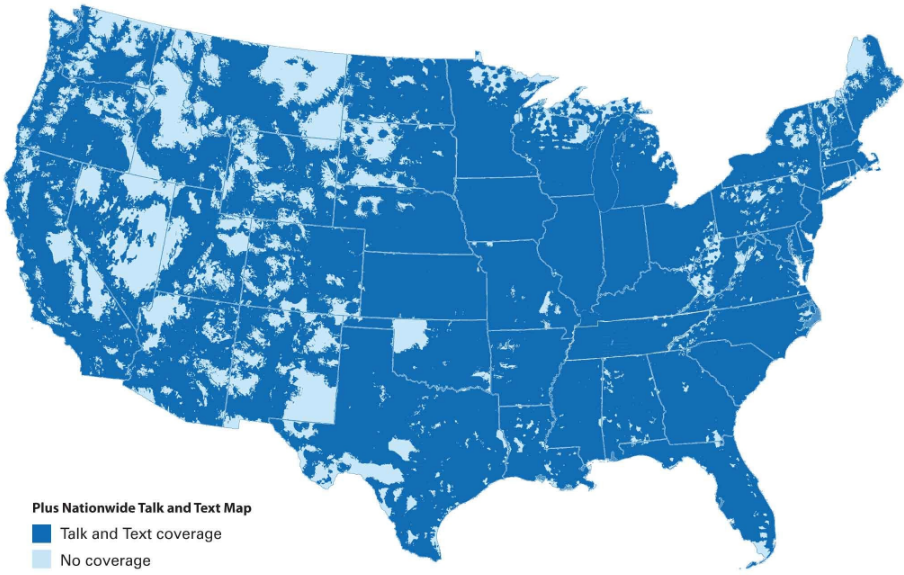
\includegraphics[width=0.7\textwidth]{images/att-coverage.png}
    \caption{Mappa compertura AT\&T negli USA}
\end{figure}\\
La loro struttura e architectura hanno subito numerosi cambiamenti nel corso delle generazioni, in particolare con la rete
5g. Si possono comunque identificare degli elementi chiave che sono presenti in tutte le generazioni:
\begin{itemize}
    \item UE \textit{User Equipment} ovvero il dispositivo cellulare
    \item RAN \textit{Radio Access Network} ovvero l'infrastruttura fisica di antenne per la ricezione e trasmissione di informazioni per il dispositivo
    \item \textit{Mobile Core} ovvero i componenti della sua architettura
\end{itemize}
\begin{figure}[h]
    \centering
    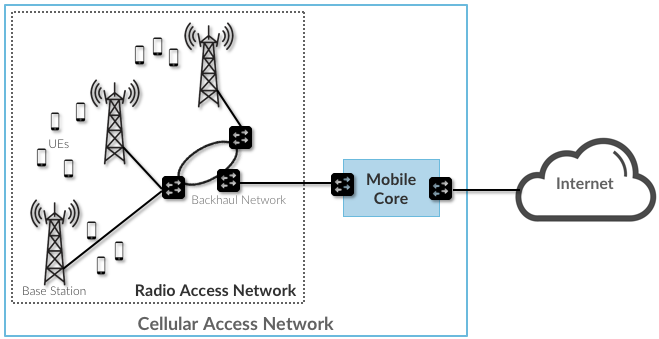
\includegraphics[width=0.7\textwidth]{images/cellular-network-basic-scheme.png}
    \caption{Schema di una rete cellulare}
\end{figure}

\section{Infrastruttura}
Per rendere possibile il collegamento di dispositivi in zone molto vaste vengono usati i ripetitori di segnale chiamati \textit{base station}. 
Questi vengono disposti in modo capillare sul territorio, suddividendolo in diverse aree di competenza chiamate celle. Ognuna di queste può gestire
un numero limitato di dispositivi in contemporanea, che chiameremo \textit{mobile station}, per questo, in caso di aree densamente popolate vengono 
ridotte le aree di competenza di ciascuna antenna. Le celle quindi, possono avere una dimensione variabile che dipende dal contesto in cui devono essere inserite.
%Immagine scacchiera cellulare
\begin{figure}[h]
    \centering
    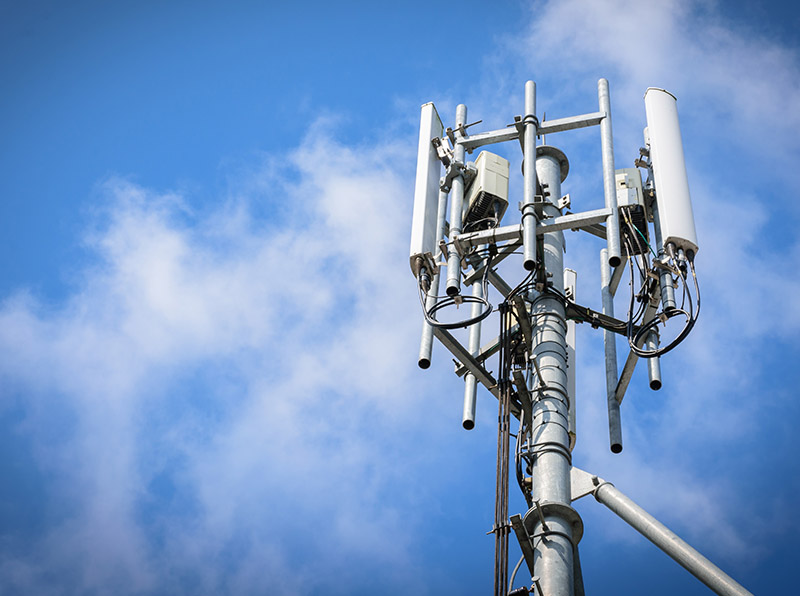
\includegraphics[width=0.5\textwidth]{images/base-station.jpg}
    \caption{Base station}
\end{figure}\\
Ogni cella ha un determinato raggio di azione che dipende dalle caratteristiche fisiche dell'antenna stessa. Inoltre, 
ha a disposizione un determinato range di frequenze su cui instaurare la comunicazione con i vari dispositivi, che solitamente
sono differenti rispetto a quelle usate dalle celle vicine per evitare interferenze.
Celle sufficientemente distanti possono utilizzare le stesse frequenze poiché non corrono il rischio di interferenza, questo rappresenta
un grande vantaggio per questa tecnologia.
\begin{figure}[h]
    \centering
    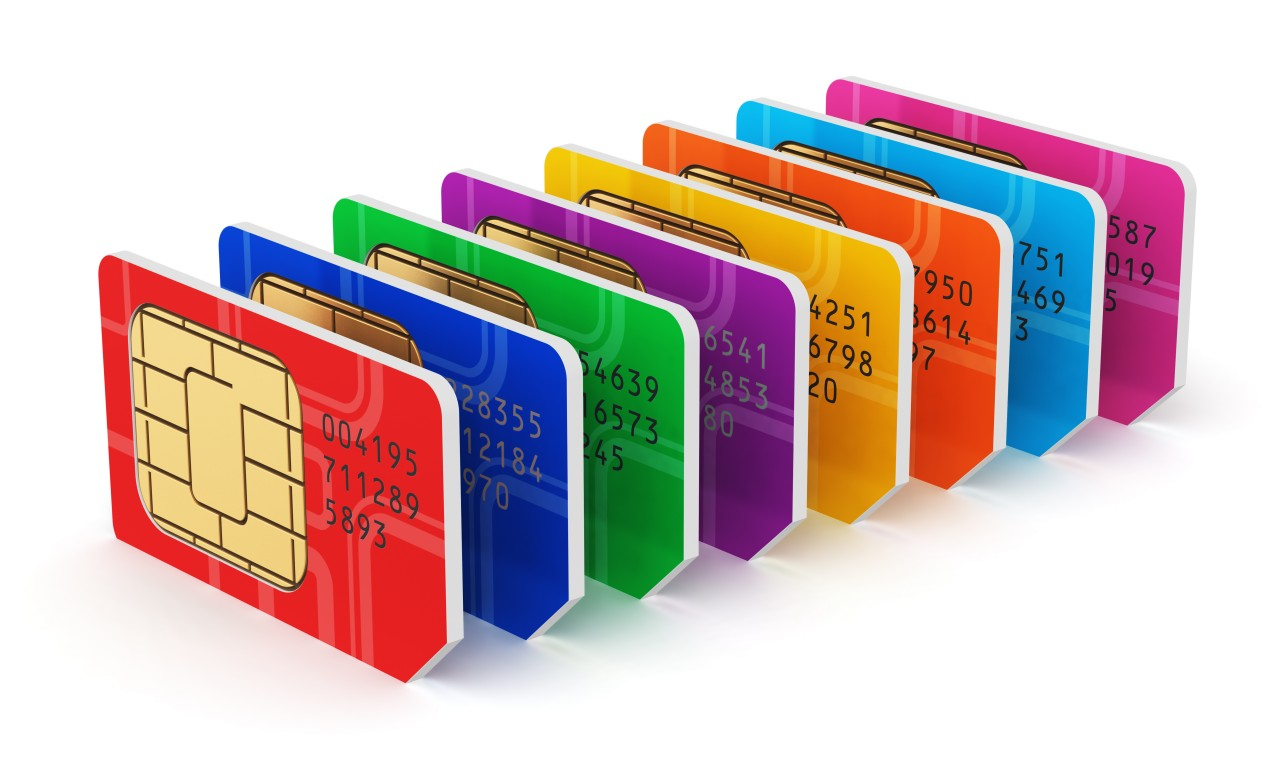
\includegraphics[width=0.5\textwidth]{images/simcard.jpg}
    \caption{SIM \textit{Subscriber Identity Module}}
\end{figure}

\section{Architettura}
L'architettura di una rete cellulare può essere risassunta con alcuni fondamentali componenti. La \textit{mobile sation} si connette all'antenna
della zona di competenza ossia la \textit{base transceiver station}, quest'ultima quando riceve l'informazione la inoltra alla rispettiva \textit{base station controller}, ossia
un componente che si occupa di raggruppare diverse \textit{base station}. 
Diversi \textit{BSC} sono raggruppati nel \textit{mobile switching centre} \gls{msc}